\documentclass[11pt]{article}
\usepackage[margin=1in]{geometry}
\usepackage{graphicx}
\usepackage{float}
\usepackage{booktabs}
\usepackage{siunitx}
\usepackage{amsmath}
\usepackage{amssymb}
\usepackage{pgfplots}
\pgfplotsset{compat=1.18}

\title{Lab 15 ECG Circuit – Analog Filtering and A/D Conversion\\
  and\\
  Lab 16 Digital Signal Manipulation of the ECG Signal
}
\author{Sean Balbale}
\date{December 7th, 2024}
\setlength{\parindent}{0in}
\setlength{\parskip}{\baselineskip}

\begin{document}

\begin{titlepage}
  \begin{center}
    \vspace*{1in}

    \Huge
    \textbf{Labs 15 and 16}

    \LARGE
    ECG Circuit – Analog Filtering and A/D Conversion and Digital Signal Manipulation of the ECG Signal

    \vspace{3in}

    \textbf{Student Name:} Sean Balbale
    \\ \textbf{Instructor:} Dr. Iman Salama
    \\ \textbf{Lab Partner Name:} Krish Gupta
    \\ \textbf{Date:} December 7, 2024

    \vfill

  \end{center}
\end{titlepage}

\newpage

\section{Introduction}
The ability to accurately record and analyze electrocardiogram (ECG) signals is critical in medical diagnostics and
health monitoring. An ECG signal provides detailed insights into the electrical activity of the heart, and any distortion
or noise can impact the reliability of the diagnosis. This project, spanning Labs 15 and 16, focused on developing an
integrated analog and digital system for processing ECG signals.

Lab 15 aimed to design and build an analog filtering circuit that removes unwanted noise and prepares the signal for
analog-to-digital conversion (A/D). This included implementing a high-pass filter to eliminate DC components, a low-pass
filter to suppress high-frequency noise, and optimizing the circuit to work within the constraints of the A/D converter’s
voltage range. The filtered signal was then digitized using the NI USB-6001 A/D converter for further processing.

Lab 16 extended the project into the digital domain, employing MATLAB to enhance the signal through digital filtering
techniques. Specific objectives included implementing a low-pass filter for additional noise reduction, designing a
notch filter to remove 60 Hz interference caused by power lines, and analyzing the signal to extract physiological
information such as heart rate. The project also involved developing custom MATLAB scripts to process and visualize
the ECG signals.
\section{Circuit Design}
\subsection{High-pass Filter}
The high-pass filter was designed to remove DC components from the signal, with a cut-on frequency of \SI{0.2}{\hertz} and a gain of 2. The circuit was implemented as shown in Figure~\ref{fig:highpass}. The resistor and capacitor values were calculated as:
\[
  f_c = \frac{1}{2 \pi R_f C} = \SI{0.2}{\hertz}, \quad \text{gain} = \frac{R_f}{R_s} = 2,
\]
\[
  R_s = \SI{500}{\kilo\ohm}, \quad R_f = \SI{1}{\mega\ohm}, \quad C = \SI{1.5}{\nano\farad}.
\]
\begin{figure}[H]
  \centering
  \includegraphics[width=0.5\textwidth]{photos/Active_First_Order_High_Pass_Filter.png}
  \caption{Active First Order High Pass Filter.}
  \label{fig:highpass}
\end{figure}
\subsection{Low-pass Filter}
A low-pass filter was implemented to reduce high-frequency noise with a cut-off frequency between \SI{200}{\hertz} and \SI{400}{\hertz} with a gain of 100. The circuit is shown in Figure~\ref{fig:lowpass}.

The resistor and capacitor values were calculated as:
\[
  f_c = \frac{1}{2 \pi R_f C} = \SI{300}{\hertz}, \quad \text{gain} = \frac{R_f}{R_s} = 100,
\]
\[
  R_s = \SI{2.6}{\kilo\ohm}, \quad R_f = \SI{260}{\kilo\ohm}, \quad C = \SI{2}{\nano\farad}.
\]
\begin{figure}[H]
  \centering
  \includegraphics[width=0.5\textwidth]{photos/Active_First_Order_Low_Pass_Filter.png}
  \caption{Active First Order Low Pass Filter.}
  \label{fig:lowpass}
\end{figure}
\subsection{Signal Path Design}
The complete signal path, including instrumentation amplifier, high-pass filter, and low-pass filter stages, is illustrated in Figure~\ref{fig:signalpath}.
\begin{figure}[H]
  \centering
  \includegraphics[width=0.5\textwidth]{photos/Signal_Path_for_ECG_Filtering_and_Acquisition.png}
  \caption{Signal Path for ECG Filtering and Acquisition.}
  \label{fig:signalpath}
\end{figure}
\section{Experimental Setup}
The complete circuit was assembled on a breadboard (Figure~\ref{fig:breadboard}). Proper grounding and lead placement were critical for minimizing noise and ensuring signal fidelity.
\begin{figure}[H]
  \centering
  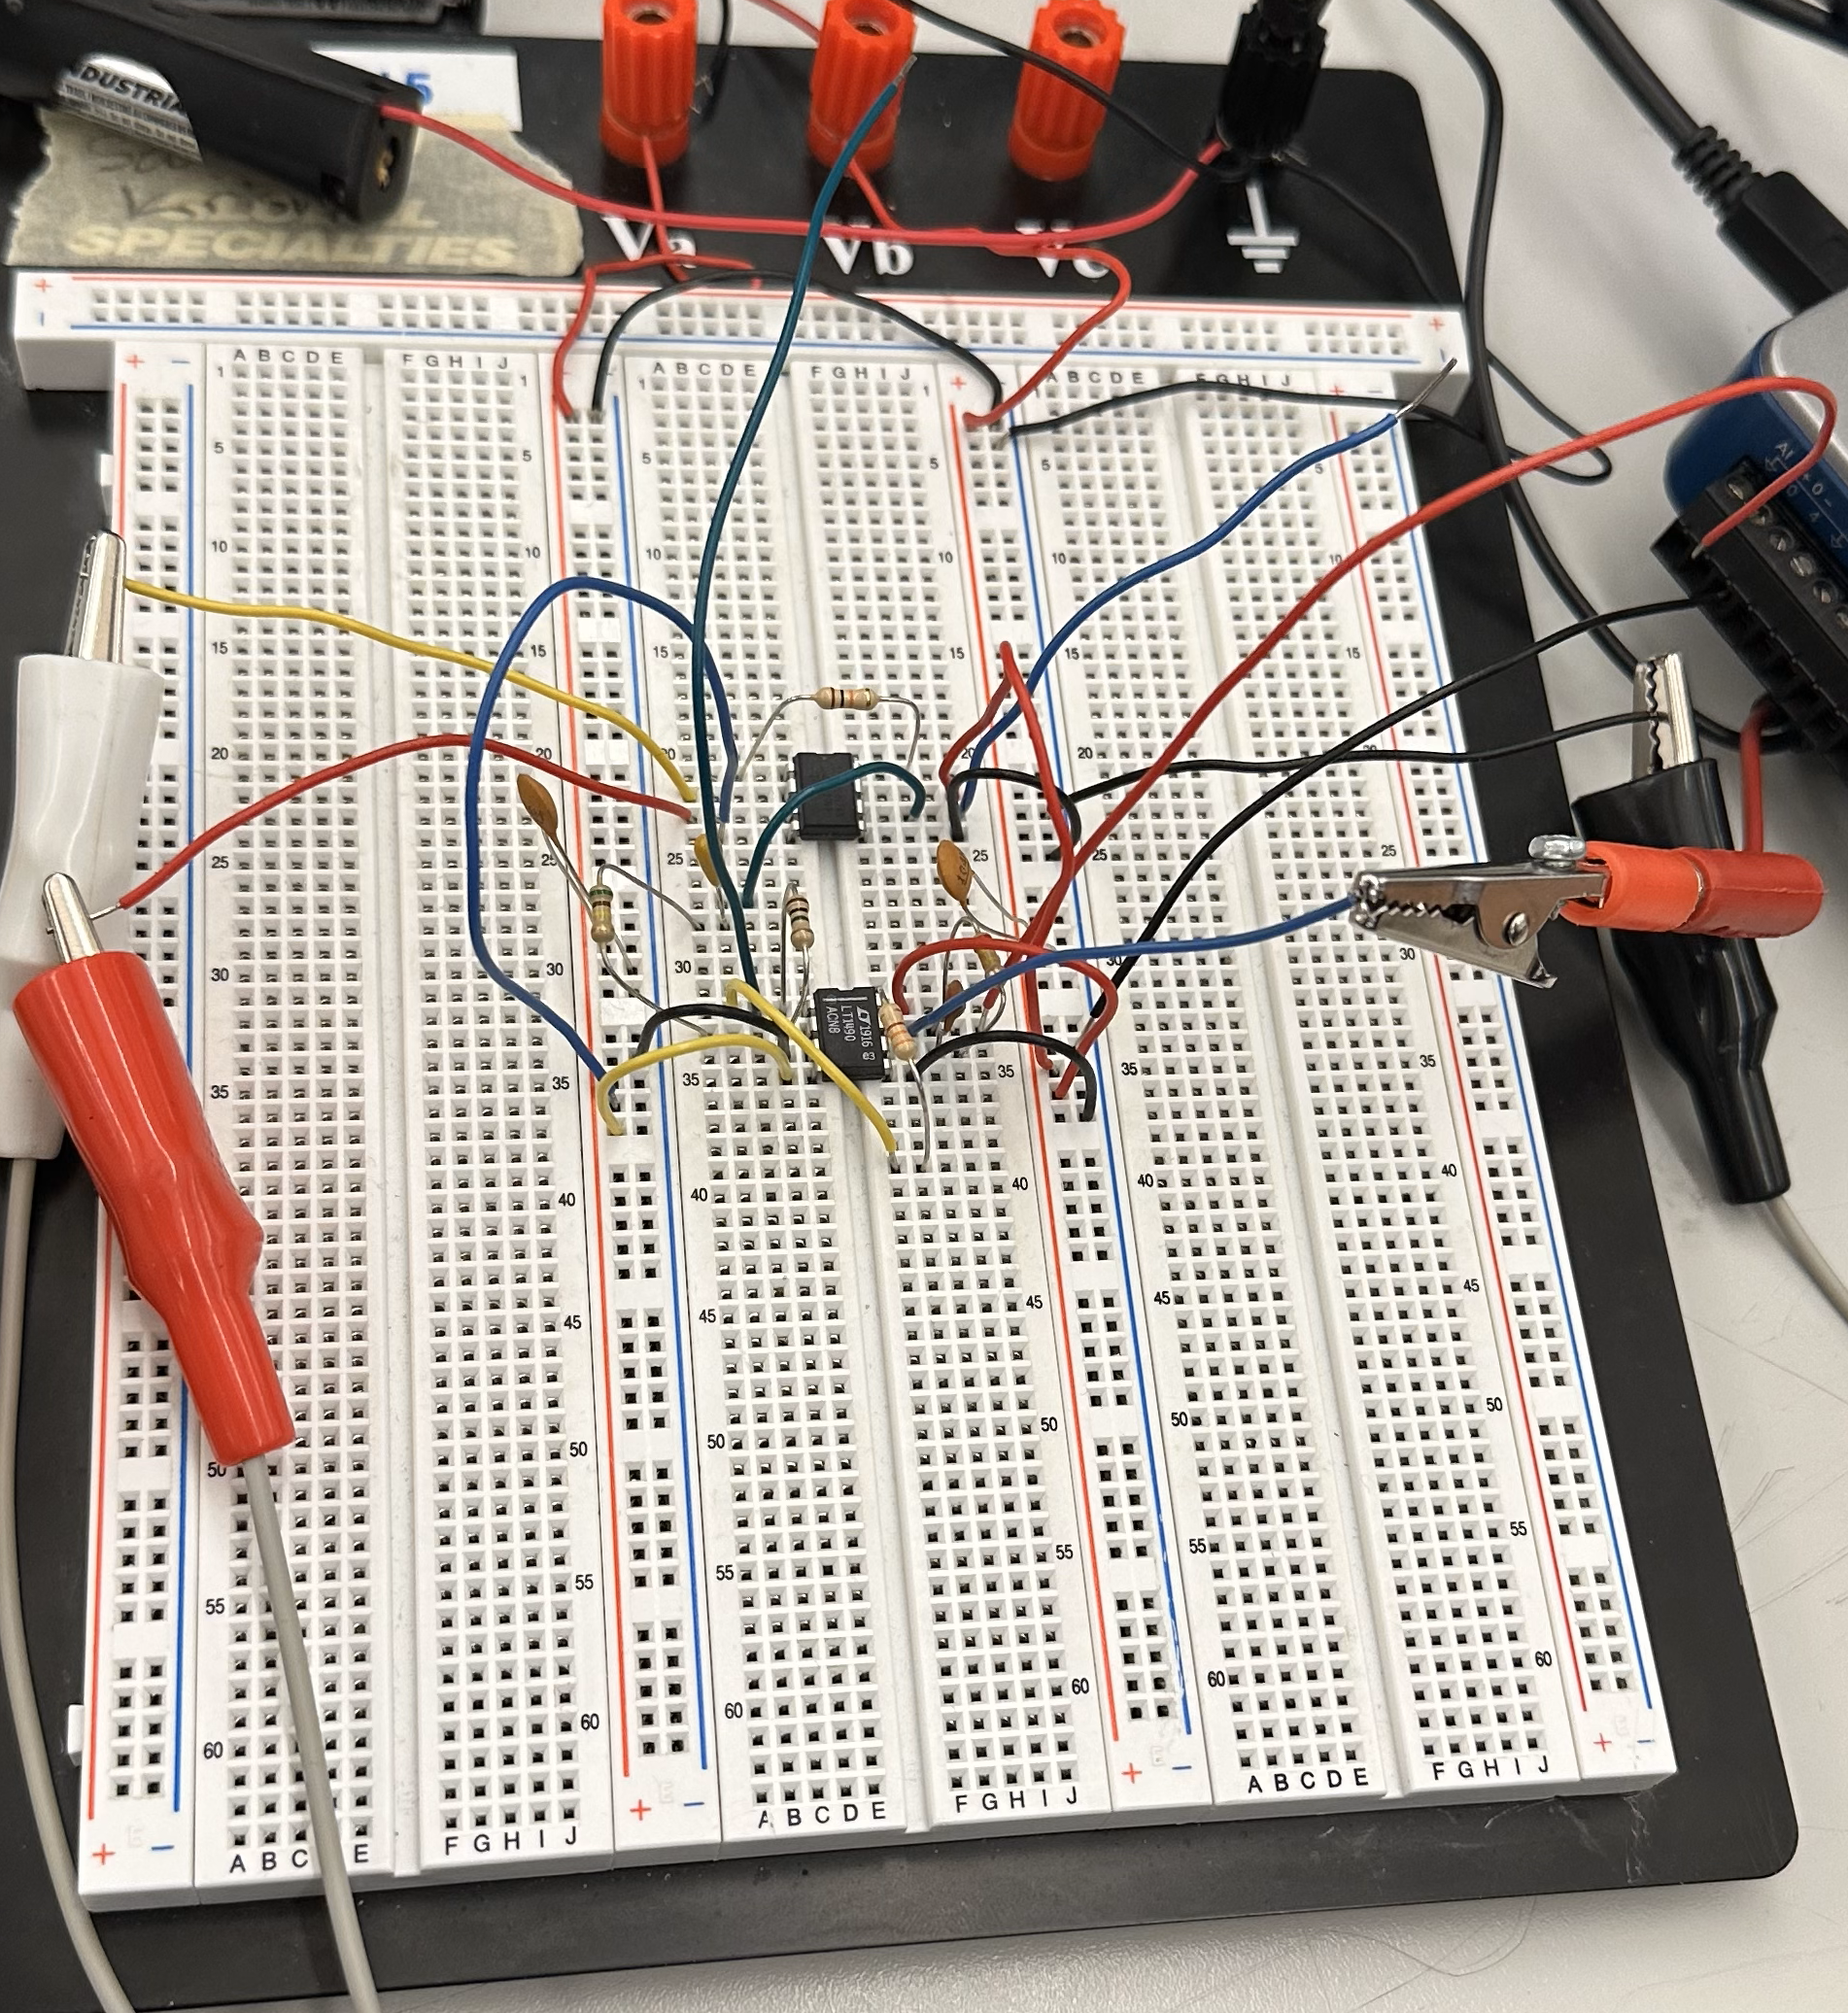
\includegraphics[width=0.5\textwidth]{photos/ECG_Circuit_On_Breadboard.png}
  \caption{ECG Circuit Assembled on a Breadboard.}
  \label{fig:breadboard}
\end{figure}
\section{Results}
\subsection{Oscilloscope Readings}
Raw and filtered ECG signals were recorded using an oscilloscope, as shown in Figures~\ref{fig:rawosc} and \ref{fig:filteredosc}.
\begin{figure}[H]
  \centering
  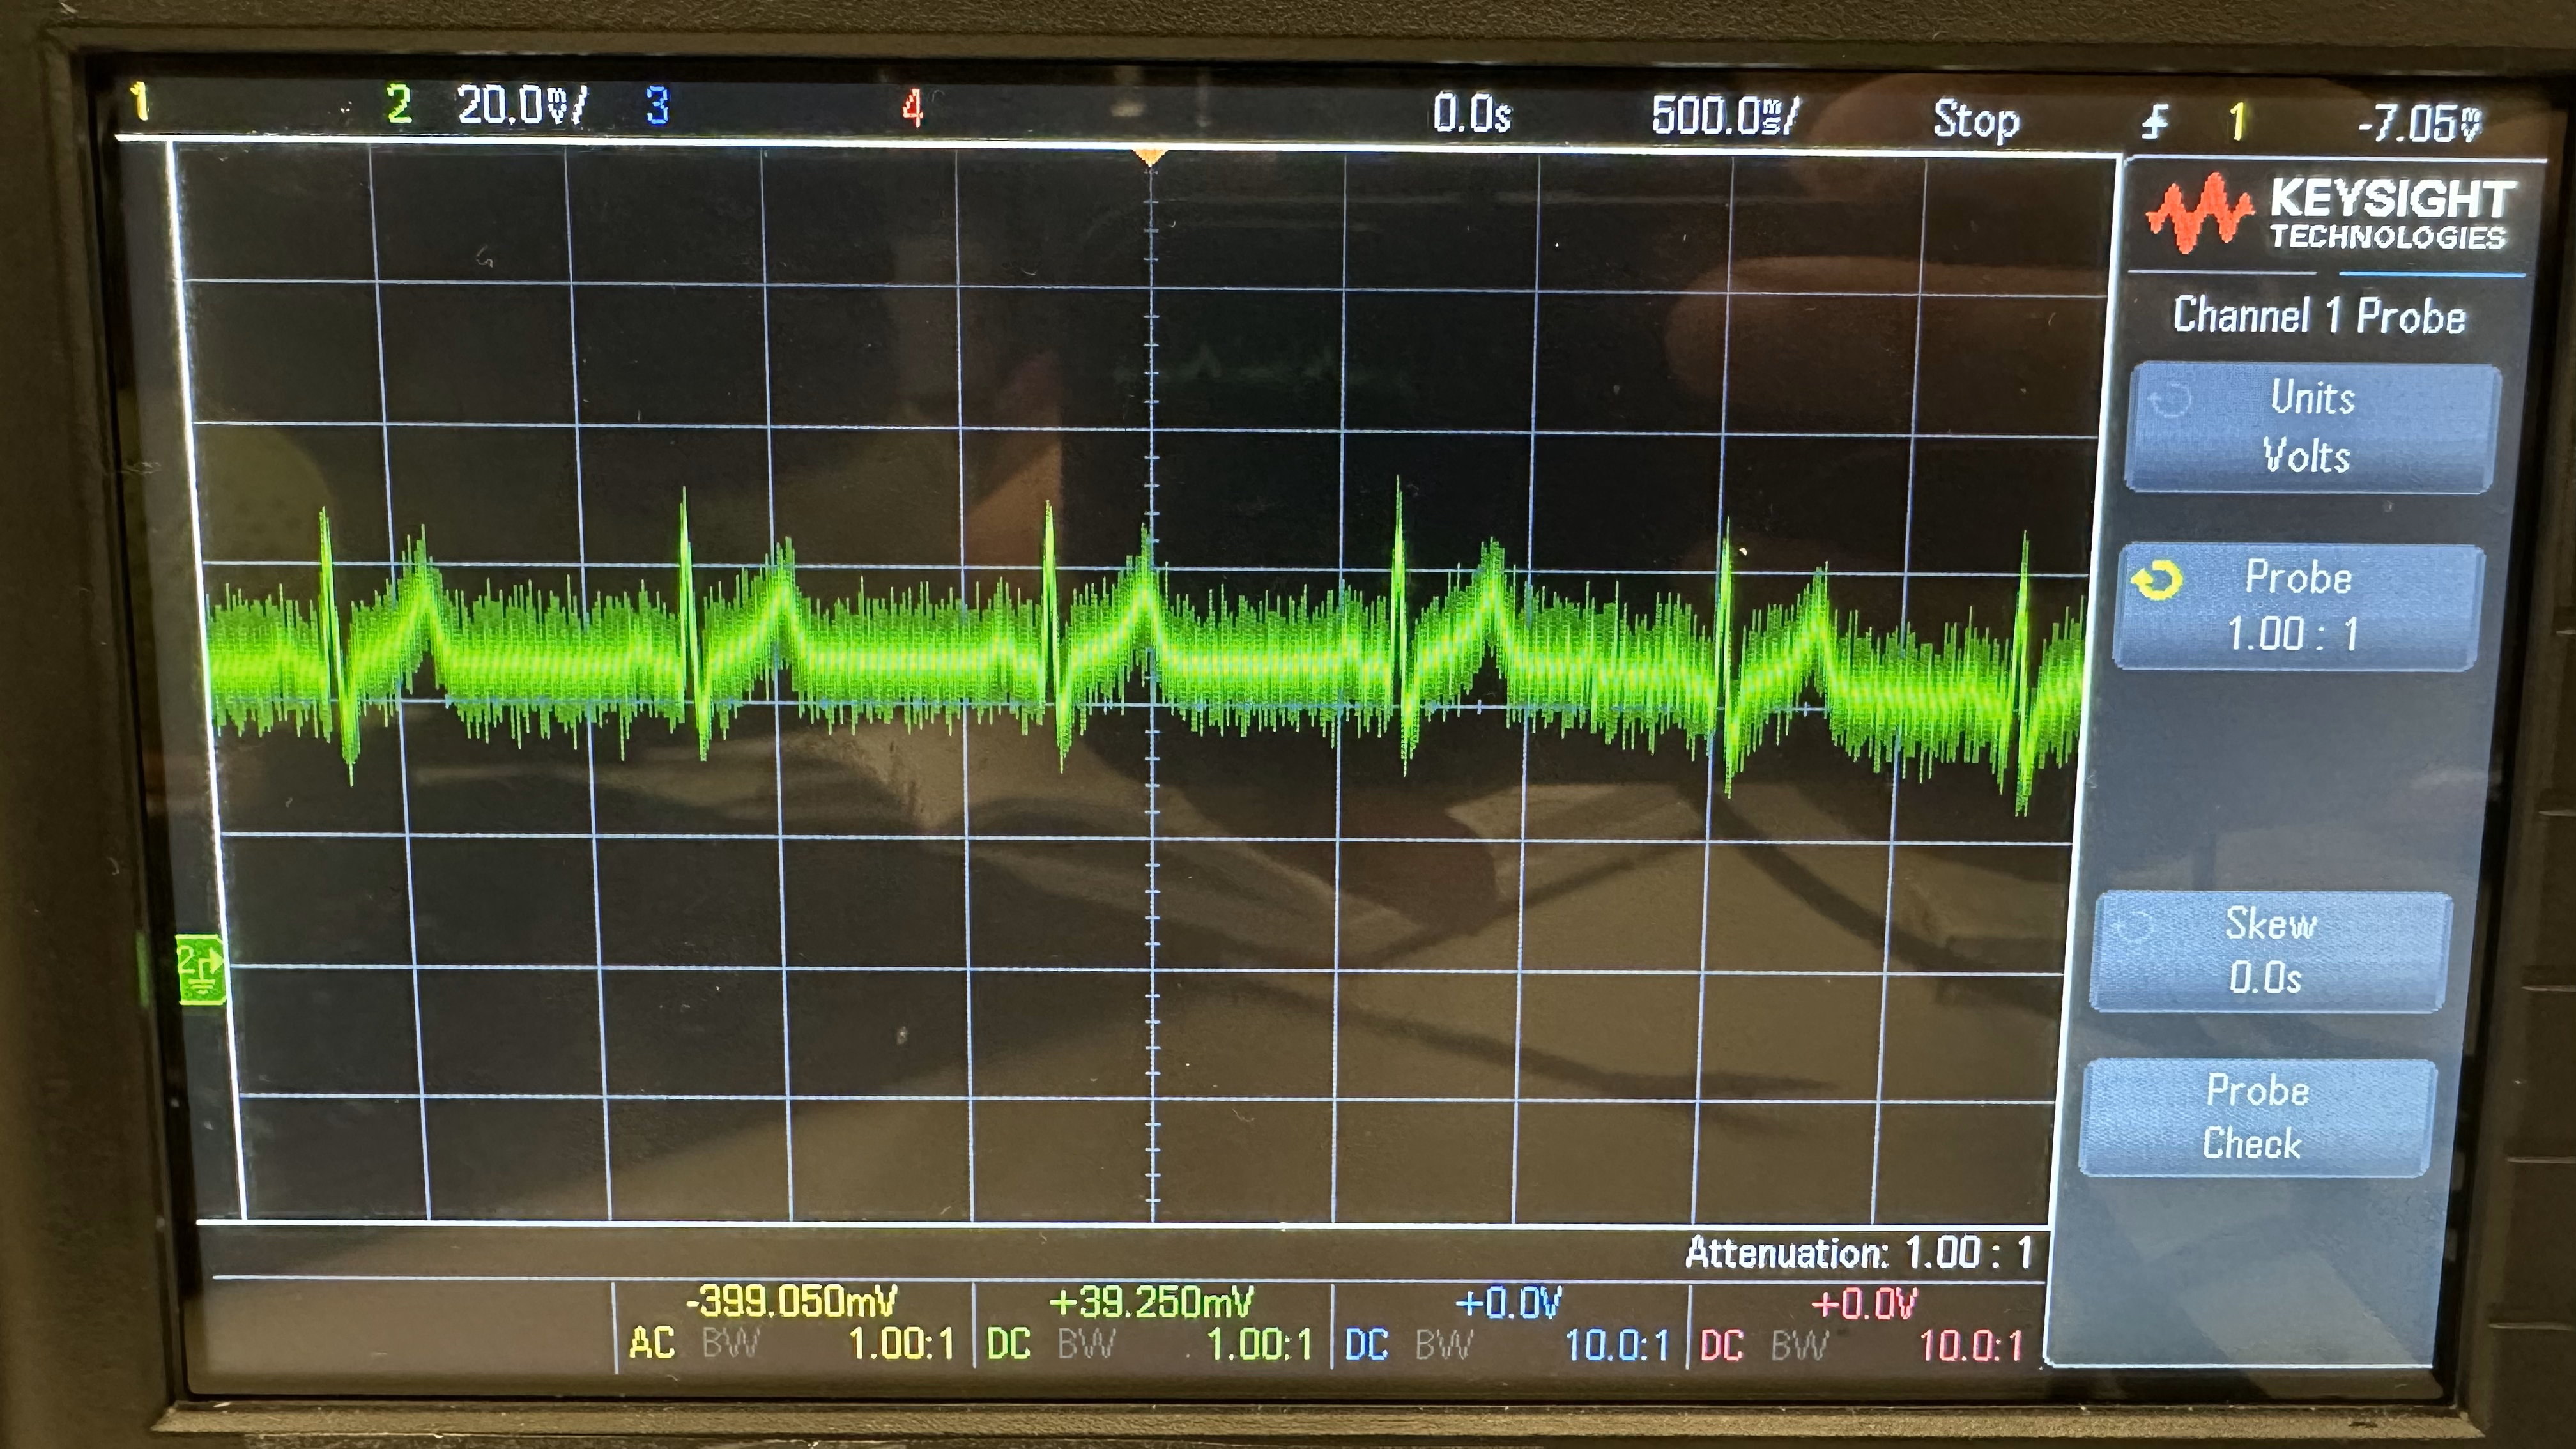
\includegraphics[width=0.75\textwidth]{photos/Raw_Oscilloscope_ECG_Output.png}
  \caption{Raw Oscilloscope ECG Output.}
  \label{fig:rawosc}
\end{figure}
\begin{figure}[H]
  \centering
  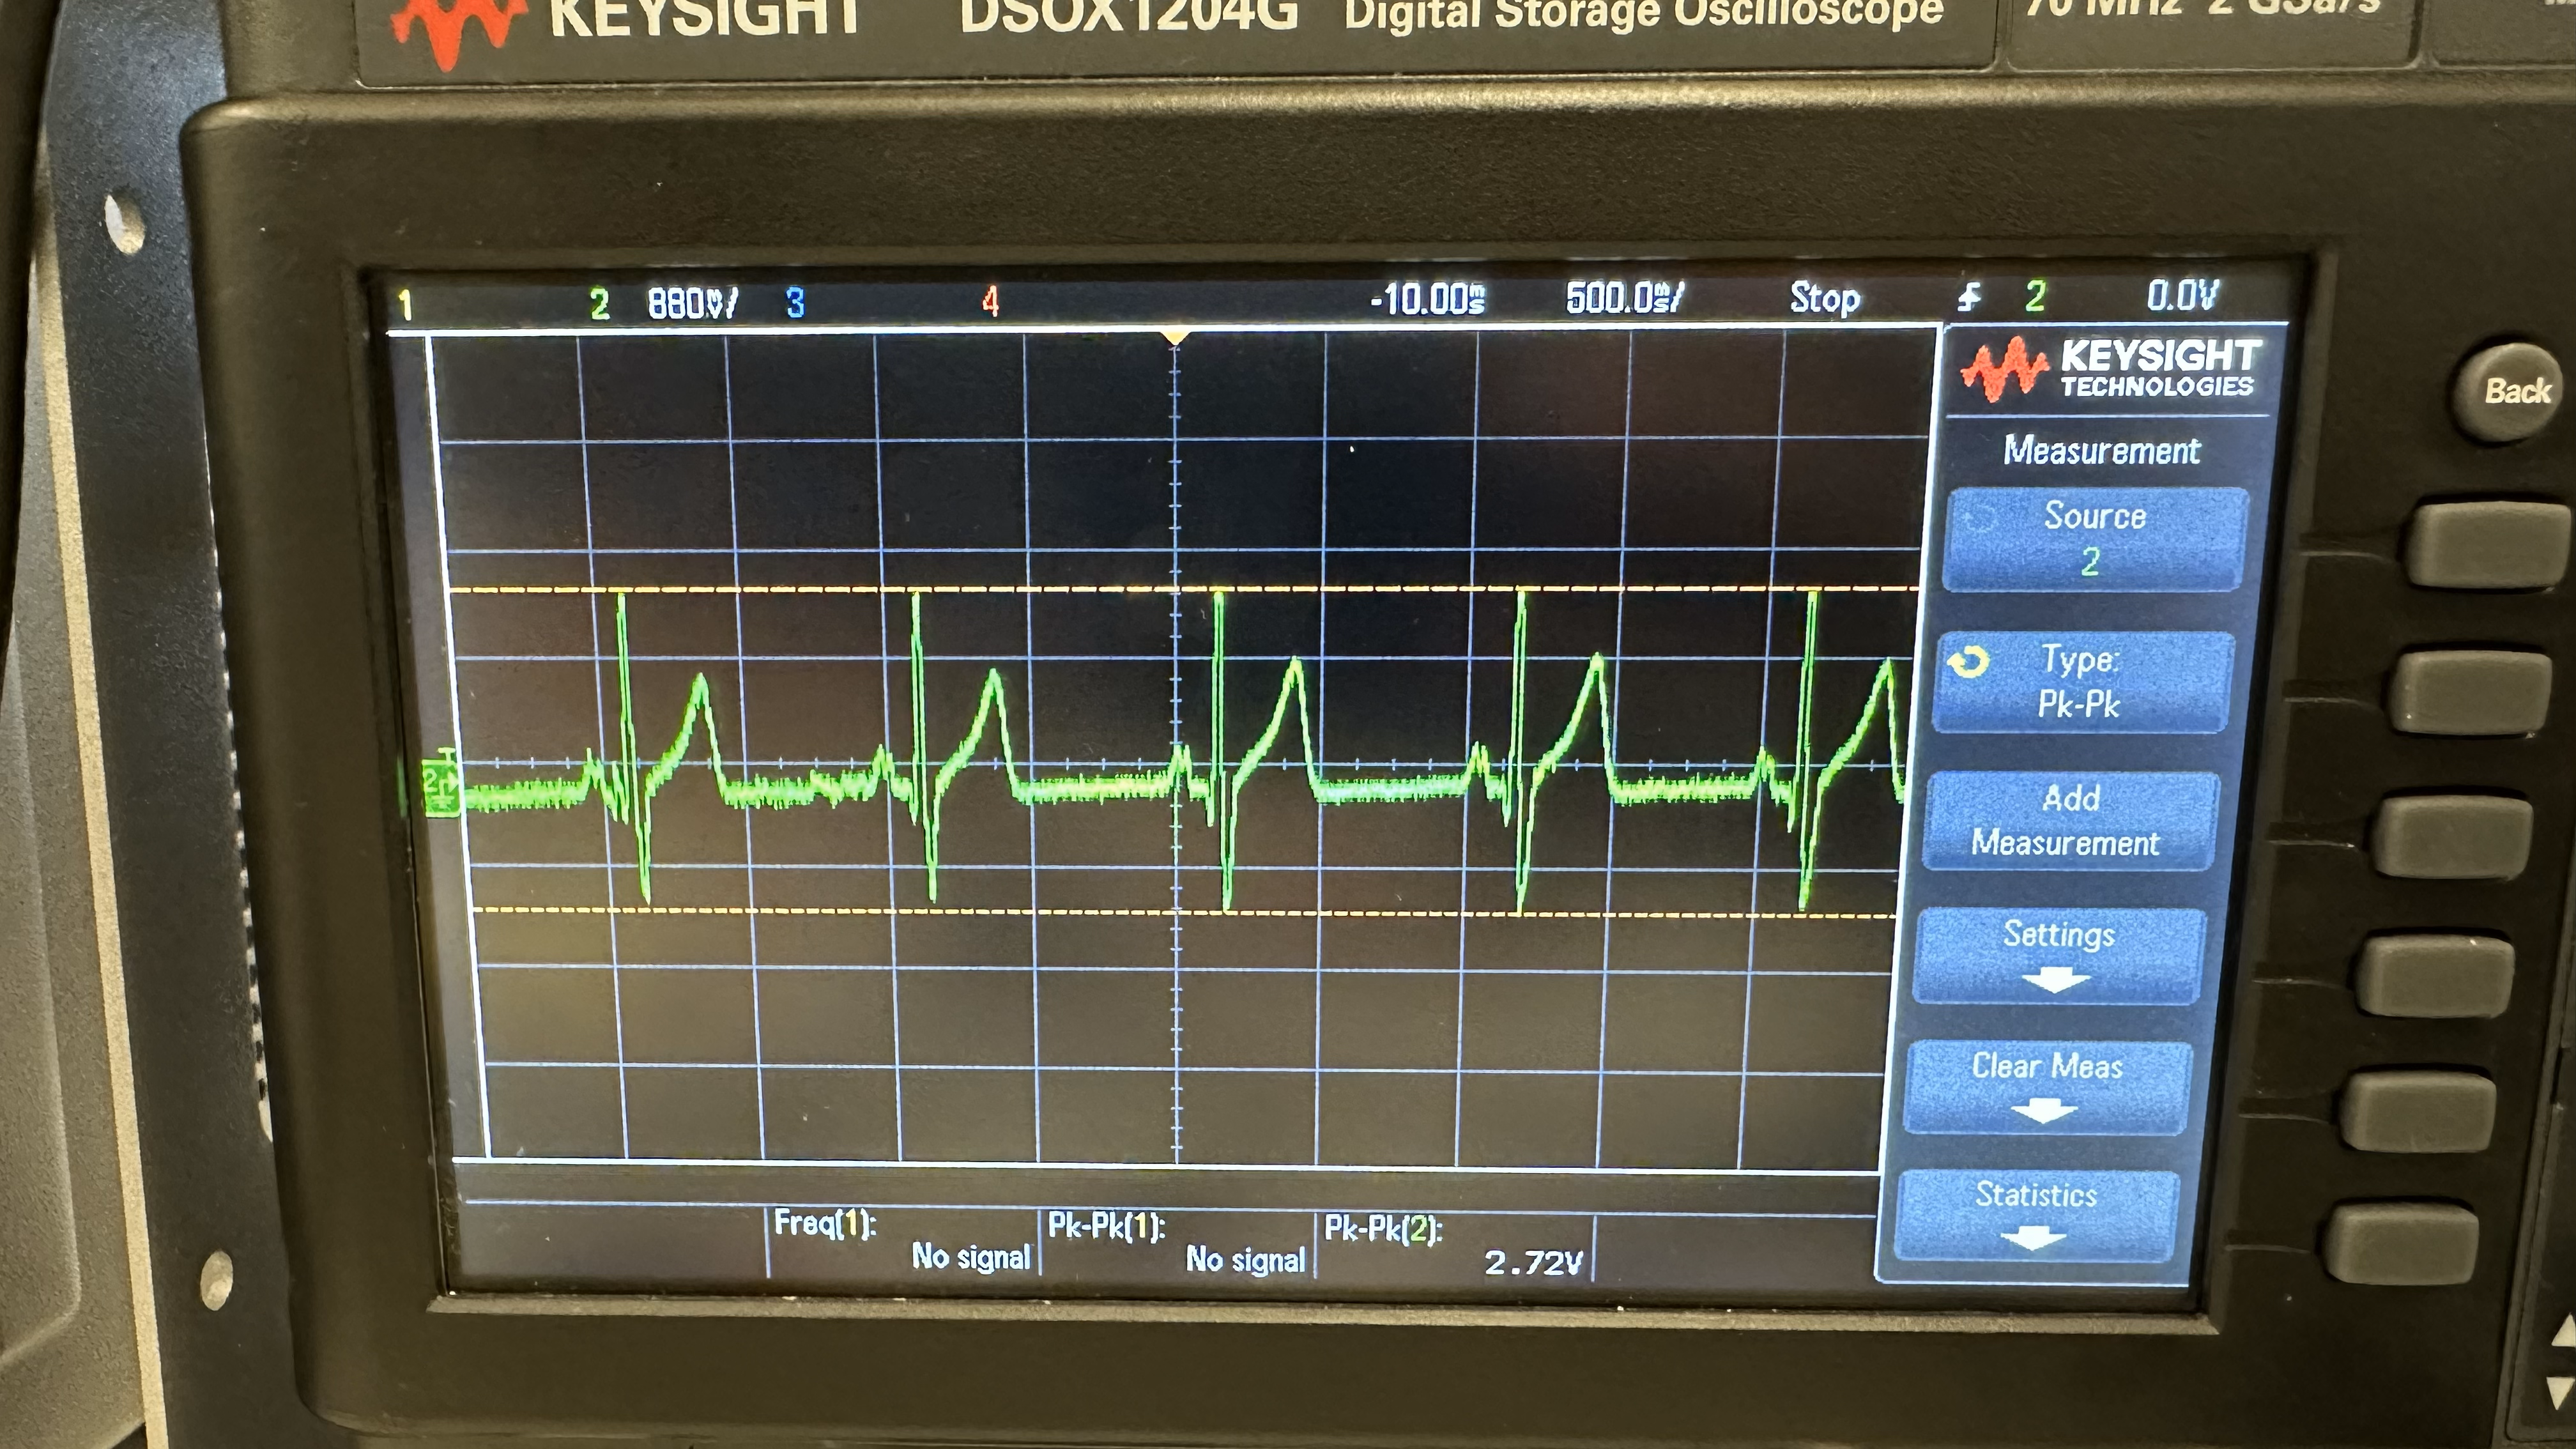
\includegraphics[width=0.75\textwidth]{photos/Filtered_Oscilloscope_ECG_Output.png}
  \caption{Filtered Oscilloscope ECG Output.}
  \label{fig:filteredosc}
\end{figure}
\subsection{Raw ECG Signals}
Raw ECG signals were recorded and displayed as shown in Figure~\ref{fig:rawsignals}.
\begin{figure}[H]
  \centering
  \includegraphics[width=0.75\textwidth]{photos/Figure_1_Raw_ECG_Signals.png}
  \caption{Raw ECG Signals.}
  \label{fig:rawsignals}
\end{figure}
\subsection{Scaled ECG Signals}
The raw signals were scaled to reflect the actual voltages at the electrodes (Figure~\ref{fig:scaledsignals}).
\begin{figure}[H]
  \centering
  \includegraphics[width=0.75\textwidth]{photos/Figure_2_Scaled_ECG_Signals.png}
  \caption{Scaled ECG Signals.}
  \label{fig:scaledsignals}
\end{figure}
\subsection{Filtered Signals}
Figures~\ref{fig:lowpassfiltered} and \ref{fig:notchfiltered} show the results of low-pass and notch filtering, respectively.
\begin{figure}[H]
  \centering
  \includegraphics[width=0.75\textwidth]{photos/Figure_5_Low_Pass_Filtered_ECG_Signals.png}
  \caption{Low-pass Filtered ECG Signals.}
  \label{fig:lowpassfiltered}
\end{figure}
\begin{figure}[H]
  \centering
  \includegraphics[width=0.75\textwidth]{photos/Figure_6_Notch_Filtered_ECG_Signals.png}
  \caption{Notch Filtered ECG Signals.}
  \label{fig:notchfiltered}
\end{figure}
\subsection{Digital Signal Processing}
MATLAB was used to process the filtered signals further. The Fast Fourier Transform (FFT) revealed a dominant 60 Hz noise,
which was effectively removed using a notch filter. A low-pass digital filter suppressed additional high-frequency noise,
and heart rate was calculated using a peak detection algorithm. Figure~\ref{fig:heartrate} shows the detected R-peaks
from the ECG signals. The calculated heart rate was approximately 63 beats per minute (BPM).
\begin{figure}[H]
  \centering
  \includegraphics[width=0.75\textwidth]{photos/Figure_7_Heart_Rate_Detection.png}
  \caption{Heart Rate Detection from ECG Signals.}
  \label{fig:heartrate}
\end{figure}
\section{MATLAB Code for Digital Signal Processing}
The MATLAB code played a pivotal role in processing and analyzing the ECG signals. The key functionalities of the MATLAB
scripts are summarized below:
\subsection{Reading and Plotting Data}
The script \texttt{Read\_Data.m} was used to import the ECG data stored in a \texttt{.mat} file and visualize the raw signals.
This allowed for a quick assessment of the signal quality and the presence of noise.
\subsection{Digital Filtering}
Two filtering techniques were implemented:
\begin{itemize}
  \item \textbf{Low-pass filtering:} A Parks-McClellan filter was implemented to suppress high-frequency noise while
    preserving the ECG signal's integrity. The design parameters were chosen based on the frequency content analysis.
  \item \textbf{Notch filtering:} A notch filter centered at 60 Hz was used to remove power line interference. The filter
    effectively attenuated the 60 Hz noise without distorting the ECG signal.
\end{itemize}
\subsection{Heart Rate Detection}
The script \texttt{Heartrate\_Recording.m} employed a peak detection algorithm to identify R-peaks in the ECG signal. These
peaks were used to calculate the heart rate in beats per minute (BPM). The results were plotted alongside the ECG signal,
clearly marking the detected peaks.
\subsection{Heartrate\_Recording.m}
The \texttt{Heartrate\_Recording.m} script is designed to accurately detect the R-peaks in the ECG signal and calculate the heart rate. The key steps in the script are as follows:
\begin{itemize}
  \item \textbf{Initialization:} The script initializes the NI USB-6001 device for data acquisition, setting the acquisition rate and duration.
  \item \textbf{Data Acquisition:} The script acquires multiple ECG signals using the NI USB-6001 device and stores the data in a cell array.
  \item \textbf{Data Storage:} The acquired ECG data is saved to a \texttt{.mat} file for later use.
  \item \textbf{Preprocessing:} The ECG signal is preprocessed to remove any baseline wander and high-frequency noise.
  \item \textbf{Peak Detection:} A peak detection algorithm is applied to identify the R-peaks in the ECG signal. This involves setting a threshold to distinguish the R-peaks from other components of the ECG waveform.
  \item \textbf{Heart Rate Calculation:} The time intervals between consecutive R-peaks are measured, and the heart rate is calculated as the number of beats per minute (BPM).
  \item \textbf{Visualization:} The detected R-peaks are plotted alongside the ECG signal, clearly marking the detected peaks and providing a visual representation of the heart rate calculation.
\end{itemize}
The script effectively identifies the R-peaks and calculates the heart rate with high accuracy, as demonstrated by the results shown in Figure~\ref{fig:heartrate}.
\section{Discussion and Conclusion}
The results of this project demonstrate the importance of a combined analog and digital approach to biomedical signal
processing. The analog filters effectively eliminated DC components and high-frequency noise, ensuring that the signal
remained within the A/D converter's dynamic range without saturation. The modularity of the design allowed for easy
debugging and tuning of individual filter stages, providing flexibility in optimizing signal quality.

In the digital domain, the MATLAB scripts further refined the signal through FFT-based analysis, low-pass filtering, and
notch filtering to remove residual noise and 60 Hz interference. The implementation of a peak detection algorithm enabled
accurate heart rate calculation, demonstrating the clinical relevance of the processed signal.

Challenges included tuning the filters to balance noise suppression with signal preservation and addressing the limitations
of the A/D converter's resolution. These were mitigated through iterative adjustments to the filter parameters and thorough
testing at each stage.

Future work could explore real-time processing capabilities using embedded systems or more advanced adaptive filtering
techniques to handle dynamic noise conditions. Additionally, integrating machine learning algorithms for automated feature
extraction from the ECG signal could enhance its diagnostic utility.

Overall, this project highlights the synergy between analog and digital signal processing techniques in achieving robust,
high-quality ECG signal acquisition and analysis.
\section{References}
[1] Dr. Iman Salama. “Lab 15 – ECG Circuit – Analog Filtering and A/D Conversion.” Northeastern University. 7 December 2024.\\

[2] Dr. Iman Salama. “Lab 16 – Digital Signal Manipulation of the ECG Signal.” Northeastern University. 7 December 2024.

\end{document}
